
\section{Text Information Retrieval}

\begin{breakbox}
\boxtitle{B-tree:}

Self-balancing, tree like a binary tree but can have more than two children. A node with r stored elements has max. r+1 children.

\begin{center}
	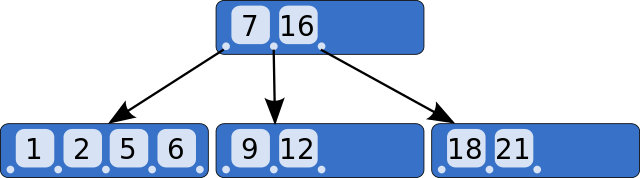
\includegraphics[width=.15\textwidth]{slides_images/b_tree_example}

\end{center}

\end{breakbox}

\begin{breakbox}
\boxtitle{Data Structure for Inverted Index:}

Usually B-trees since they are sorted. Searching for a prefix like 'hyp\%' is now easier since the tree can just be traversed with h->y->p and then collect all children.
\end{breakbox}

\begin{breakbox}
\boxtitle{Blocked Sort-Based Indexing (BSBI):}

Problem of inverted index so far: parse docs one at a time => cannot exploit compression tricks. Solution: Blocked sort-based indexing. Try to keep data as compressed as possible.

\begin{itemize}
	\item External sorting algorithm
	\item Sorting with fewer disk seeks. Basic idea:
		\begin{itemize}
			\item Accumulate postings for each block, sort, write to disk
			\item Then merge the blocks into one long sorted order		
		\end{itemize}
	\item Problem: Keeps dictionary in memory
		\begin{itemize}
			\item Answer: Single-pass in-memory indexing
		\end{itemize}
\end{itemize}
\end{breakbox}


\begin{breakbox}
\boxtitle{Distributed Index:}

\begin{itemize}
	\item Maintain a master machine directing the indexing job -- considered ''safe''
	\item Assign parallel indexing tasks to an idle machine from a pool
	\item Break the input document corpus into splits (corresponding to blocks in BSBI)
	\item on distributed computing clusters which scales (individual machines are fault-prone)
\end{itemize}

Best done with MapReduce.
\end{breakbox}

\begin{breakbox}
\boxtitle{MapReduce:}

A programming (abstraction) model and an associated implementation for processing and generating large data sets.

Phases:
\begin{enumerate}
	\item Map: Each worker node calls Map() for filtering and sorting his own data
	\item Global master node orchestrates that for redundant copies of input data, only one is processed.
	\item Shuffle: Worker nodes redistribute data based on the output keys (produced by the "map()" function), such that all data belonging to one key is located on the same worker node.
	\item Reduce: Worker nodes now process each group of output data, per key, in parallel.
\end{enumerate}

Example for counting words in documents:
\java{java_code/mapreduce_count_words.pseudo}
\end{breakbox}

\begin{breakbox}
\boxtitle{Statistics from Preprocessing:}

\begin{itemize}
	\item Stemming and case folding reduce the indexed terms about 17\,\%.
	\item 30 most common words account for 30\,\% of the tokens in written text.
\end{itemize}
\end{breakbox}

\begin{breakbox}
\boxtitle{Heaps' Law:}

Law, which describes the number of distinct words in a document as a function of the document length (so called type-token relation).

M=size of the vocabulary, T=number of tokens in collection:
\begin{center}
	$M=kT^b$
\end{center}

Typical values: $30 \leq k \leq 100$ and $b \approx 0.5$
\end{breakbox}

\begin{breakbox}
\boxtitle{Zipf's Law:}

Law for the relative frequencies of terms. In natural language, there are a few very frequent and very many very rare terms.

\begin{center}
	The $i$-th most frequent term has frequency proportional to $\frac{1}{i}$.
\end{center}

If the terms are sorted by their frequency, then their probability is inversely proportional to their position in the ordering.

$cf_i$ is collection frequency: the number of occurences of the term $t_i$ in the collection. So if the most frequent term (the) occurs $cf_1$ times
\begin{itemize}
	\item then the second most frequent term (of) occurs
$\frac{cf_1}{2}$times
	\item the third most frequent term (and) occurs $\frac{cf_1}{3}$ times \ldots
\end{itemize}m
\end{breakbox}

\begin{breakbox}
\boxtitle{IR Models -- Basic Concepts:}

\begin{itemize}
	\item Not all terms are equally useful for representing the document content: less frequent terms allow identifying a narrower set of documents
	\item Importantce of index terms is represented by weights associated to them.
	\item $ki$=index term, $d_j$=document $w_{ij}$=weight associated with $(k_i,d_j)$
	\item $w_{ij}$ quantifies the importance of the index term for describing the document contents
	\item $w_{ij}=0$ indicates that term does not belong to doc
	\item t is the total number of docs
	\item $K=(k_1,k_2, \ldots, k_t)$ set of all index terms
	\item $\text{vec}(d_j) = (w_{1j}, w_{2j}, \ldots, w_{tj})$ is a weighed vector associated with the document $d_j$
	\item $g_i(\text{vec}(d_j)) = w_{ij}$ is a function which returns the weight associated with pair $(k_i, d_j)$
\end{itemize}
\end{breakbox}

\begin{breakbox}
\boxtitle{Boolean Model:}

Queries are specified as boolean expressions. Terms are either present or absent: $w_{ij} \in {0,1}$ and \textbf{cannot match partially}.

\begin{center}
	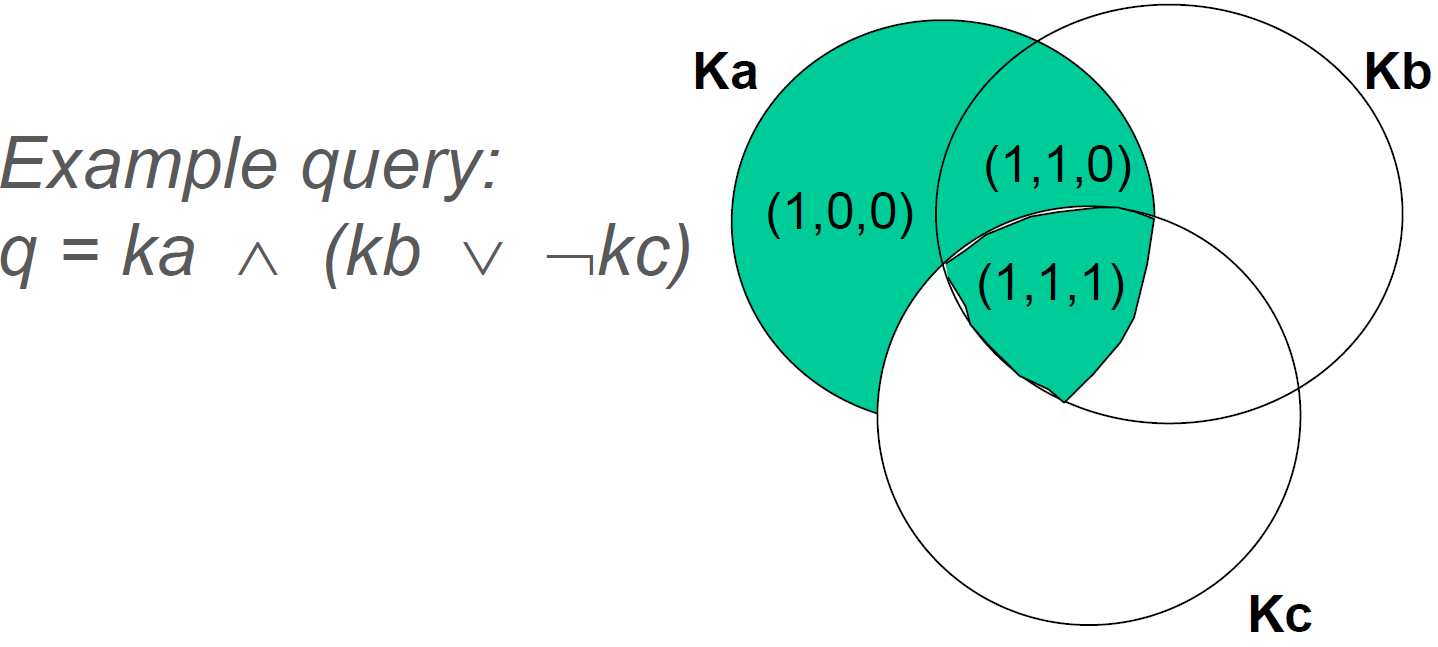
\includegraphics[width=.12\textwidth]{slides_images/boolean_model_example}
\end{center}

Disadvantages:
\begin{itemize}
	\item No ranking of the documents is provided (absence of a grading scale)
	\item Information need has to be translated into a
Boolean expression which most users find awkward
	\item Boolean queries formulated by the users are mostly too simplistic
	\item Consequence, model frequently returns either too few or too many documents in response to a user query
\end{itemize}

\end{breakbox}
\boxtitle{Vector Space Model}

\begin{breakbox}